%==================================Kapitola: Konverze mezi digitálním a analogový signálem====================
\chapter{Konverze mezi digitálním a analogový sig\-ná\-lem}
\minitoc
\newpage
\section{Konverze mezi digitálním a analogový signálem}
  Při zpracování analogového signálu je jednou z důležitých funkcí převod tohoto signálu z analogové podoby do číslicové a naopak. Proto jsou analogově-číslicové převodníky resp. číslicově-analogové převodníky (ADC - Analog-to-Digital Converter), (DAC - Digital-to-Analog Converter) velmi důležitými prvky jakéhokoli systému zpracovávajícího signál \cite[s.~11]{Haze}. Na obrázku \ref{AES:fig_ADC_DAC_IO} je definováno rozhraní obou typů převodníku.
  \begin{figure}[ht!]
     \centering
     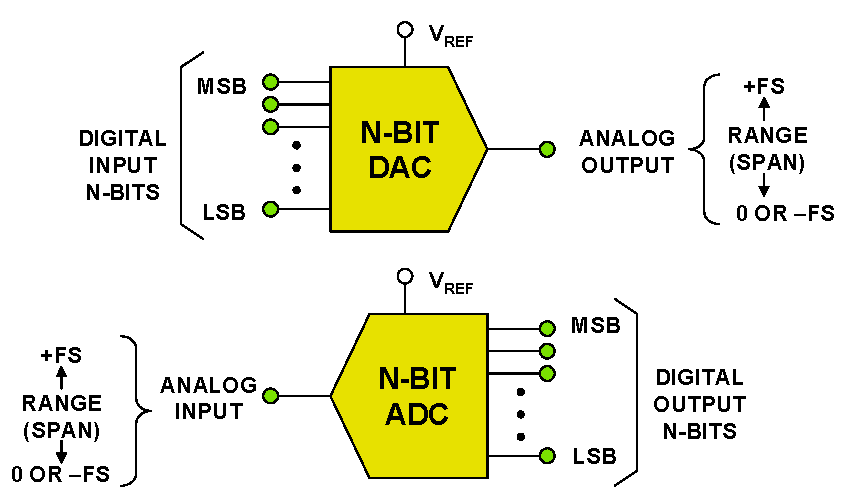
\includegraphics[width=\linewidth]{ADC_DAC_block.pdf}
     \caption[Definice I/O bloku DAC a ADC ]{Definice rozhraní bloku analogově-číslicového (ADC) a číslicově-analogového (DAC) převodníku}
     \label{AES:fig_ADC_DAC_IO}
  \end{figure}

  \textbf{Analogově-číslicové převodníky} (Analog-to-Digital Converters) slouží k pře\-ve\-de\-ní analogového 
  signálu na signál číslicový. Pro A/D převodník má analogová stupnice vstupního signálu délku \texttt{FS} 
  (\emph{Full scale}), udávanou např. ve voltech. Stupnice číslicového signálu pak vyznačuje diskrétní 
  hodnoty výstupu, které převodník generuje při převodu analogového signálu \cite[s.~202]{Neumann}.

  \textbf{Číslicově-analogové převodníky} (Digital-to-Analog Converters) slouží k o\-pač\-né\-mu procesu, 
  tedy k pře\-ve\-de\-ní číslicového signálu na signál analogový, což by šlo realizovat pomocí lineárního 
  digitálního potenciometru a připojeného zdroje referenčního napětí na jeho vstupu \cite[s.~208]{Neumann}. 
  Pro N-bitové binární slovo by musel mít $n-1$ rezistorů a $n$ resp. $2n - 1$ spínačů. To je monoliticky 
  téměř nerealizovatelné již pro osmi- a vícebitové slovo. Řešení převodníků proto musí být mnohem 
  úspornější, i když úspory budou vykoupeny jinými nevýhodami, případně omezeními pro jejich použití.

    \subsection{Základní struktura převodníků}
      Obě skupiny převodníků mohou typicky obsahovat komparátory, číslicové obvody, spínače, integrátory,  
      vzorkovací obvody a/nebo pasivní součástky. Nezbytnou a důležitou součástí je i přesný zdroj 
      referenčního napětí. V mnoha případech pak také platí, že DAC je jednou z částí ADC.
      
      Analogově číslicový převod můžeme pomyslně rozložit do tří etap \cite{Sebesta}.
      \begin{enumerate}
        \item Převod signálu se spojitým časem na signál s diskrétním časem. Tomuto převodu říkáme vzorkování.
        \item Kvantování vzorku s cílem vyjádřit vzorky konečnou množinou čísel. Tento krok je provázen    
              vznikem tzv. kvantovacího šumu. Uvedený jev souvisí s nelineárním zkreslením známým z teorie 
              obvodů.
        \item Kódování spočívající zpravidla v binárním vyjádření čísel představujících velikosti vzorku.
      \end{enumerate}
      
    \subsection{Statické a dynamické parametry převodníků}
      Statické parametry převodníků jsou určovány pomocí \emph{převodní charakteristiky}, zatím co dynamické vlastnosti se vyhodnocují z kmitočtového spektra převodníku \cite[s.~11]{Haze}.
      \begin{itemize}
        \item rozsah,
        \item integrální a diferenciální nelinearita (\emph{integral - INL, differential - DNL nonlinearity}),
        \item rozlišení převodníku (\emph{resolution}),
        \item přesnost (\emph{accuracy}),
        \item chyba monotónnosti,
        \item chyba nastavení nuly (\emph{offset error}),
        \item hystereze a další.
       \end{itemize}
       K hlavním dynamickým parametrům patří
       \begin{itemize}
         \item odstup signál - šum (\emph{signal to noise ratio - SNR}) kap. \ref{AES:cap_SNR},
         \item efektivní počet bitů (\emph{effective number of bits - ENOB}),
         \item harmonické zkreslení (\emph{total harmonic distortion - THD}),
         \item odstup signál-šum a zkreslení (\emph{signal to noise and distortion - SINAD}),
         \item dynamický rozsah bez parazitních složek \newline(\emph{spurious free dynamic range - SFDR}),
         \item šum - vrcholový, efektivní (\emph{noise - peak, rms}),
         \item doba přepnutí a ustálení.
       \end{itemize}

    \subsection{Vzorkování}
    \subsection{Kvantování}
       Pro přechod od časově spojitého signálu se spojitou množinou hodnot k číslicovému signálu, je nutné 
       provést (výškové) \texttt{kvantování}, tj. kvantování hodnot signálu, které je patrné z obrázku  
       \ref{AES:fig_Quntized_sig_wave}. Je zřejmé, že mapování spojitého intervalu vstupních
       hodnot na diskrétní hodnoty digitálního výstupu způsobí, že každá hodnota digitálního výstupu platí 
       pro vstupní signál měnící se v určitém  podintervalu. Délka podintervalu, pro který platí jedna 
       hodnota digitálního výstupu se nazývá \textbf{kvantizační krok převodníku} - \emph{Q}, jenž je roven 
       bitu s nejnižší váhou - \texttt{LSB}.

       \begin{figure}[ht!]
         \centering
         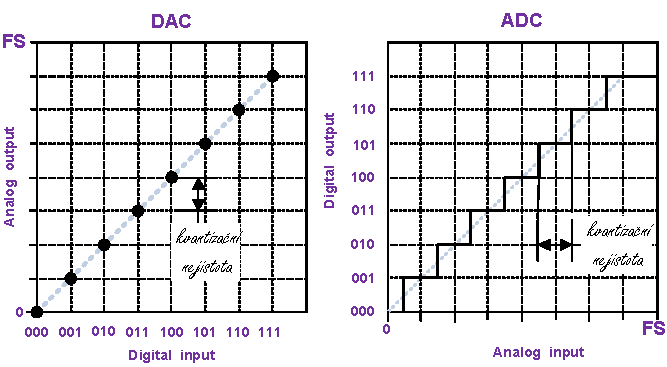
\includegraphics[width=1\linewidth]{ADC_DAC_3bit.pdf}
         \caption[Přenosová funkce AD a DA převodníku]{Ideální přenosová funkce 3bitového unipolárního AD 
                  a DA převodníku. V případě DA převodníku je přenosová funkce tvořena osmi body, nikoliv 
                  čárou.}
         \label{AES:fig_3b_DAC_ADC}
       \end{figure}
 
       Převodní charakteristika DA i AD převodníku je znázorněna na obr. \ref{AES:fig_3b_DAC_ADC}. Analogový 
       signál je spojitý a číslicový signál vyjadřuje jen jeho vybrané diskrétní hodnoty. Proto je převodní 
       charakteristika nespojitá. Naproti tomu digitální vstup vytvoří na výstupu pouze omezený počet hodnot 
       výstupního signálu.

       \begin{figure}[ht!]
         \centering
         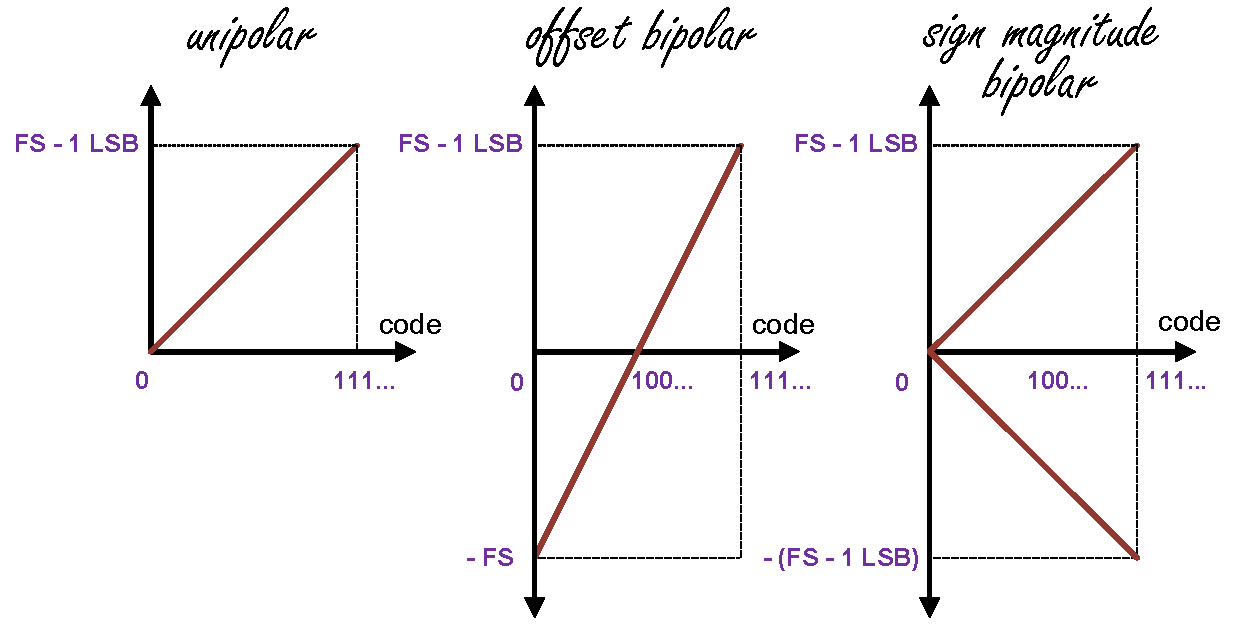
\includegraphics[width=1\linewidth]{Uni_Bi_Converter.pdf}
         \caption[Unipolární a bipolární převodníky]{Unipolární a bipolární převodníky \cite{Kester2004}}
         \label{AES:fig_uni_bi_converter}
       \end{figure}

       Počet úrovní AD převodníku, do kterého je rozdělen rozsah vstupního analogového signálu definuje 
       \textbf{rozlišovací schopnost ADC} a lze ji vyjádřit různými způsoby, jak ukazuje tabulka 
       \ref{AES:tab_10b_ADC_resolution} pro 2 až 24bitového převodníku.

         \begin{table}[ht!]
           \centering
            \setlength{\tabcolsep}{5pt}
            \begin{tabular}{|c|c|c|c|c|c|}
              \hline
                \textbf{Rozlišení} & \multirow{2}{*}{$\mathbf{2^N}$} &  \textbf{Napětí} & \multirow{2}{*}{\textbf{ppm FS}}& \multirow{2}{*}{\textbf{\% FS}}&  \multirow{2}{*}{\textbf{dB FS}} \\
                         N     &           &  \textbf{10V FS} &        &             &          \\
              \hline
                       2-bit   &         4 &            2.5 V & 250000 &          25 &  -12     \\
              \hline
                       4-bit   &        16 &           625 mV &  62500 &        6,25 &  -24     \\
              \hline
                       6-bit   &        64 &           156 mV &  15625 &        1,56 &  -36     \\
              \hline
                       8-bit   &       256 &          39,1 mV &   3906 &        0,39 &  -48     \\
              \hline
                      10-bit   &      1024 &          9,77 mV &    977 &       0,098 &  -60     \\
              \hline
                      12-bit   &      4096 &          2.44 mV &    244 &       0,024 &  -72     \\
              \hline
                      14-bit   &     16384 &       610 $\mu$V &     61 &       0,061 &  -84     \\
              \hline
                      16-bit   &     65536 &       153 $\mu$V &     15 &      0,0015 &  -96     \\
              \hline
                      18-bit   &    262144 &         38 $\mu$ &      4 &      0,0004 & -108     \\
              \hline
                      20-bit   &   1048576 &       9.54 $\mu$ &      1 &      0,0001 & -120     \\
              \hline
                      22-bit   &   4194304 &       2.38 $\mu$ &   0,24 &    0,000024 & -132     \\
              \hline
                      24-bit   &  16777216 &           596 nV &   0,06 &    0,000006 & -144     \\
              \hline
           \end{tabular}
           \caption[Kvantizace: Velikost LSB]{Porovnání rozlišovací schopnosti AD převodníku s různou délkou  
                    výstupního slova. Z tabulky vyplývá, že kvantizační krok 24bitového ADC odpovídá 
                    velikosti úbytku na rezistoru $2,2 k\Omega$ při teplotě 25°C, který vzniká vlivem 
                    tepelného šumu (viz Johnsonův šum) jenž je při šířce pásma 10 kHz roven 600 nV. }
           \label{AES:tab_10b_ADC_resolution}
         \end{table}

       \begin{figure}[ht!]
         \centering
         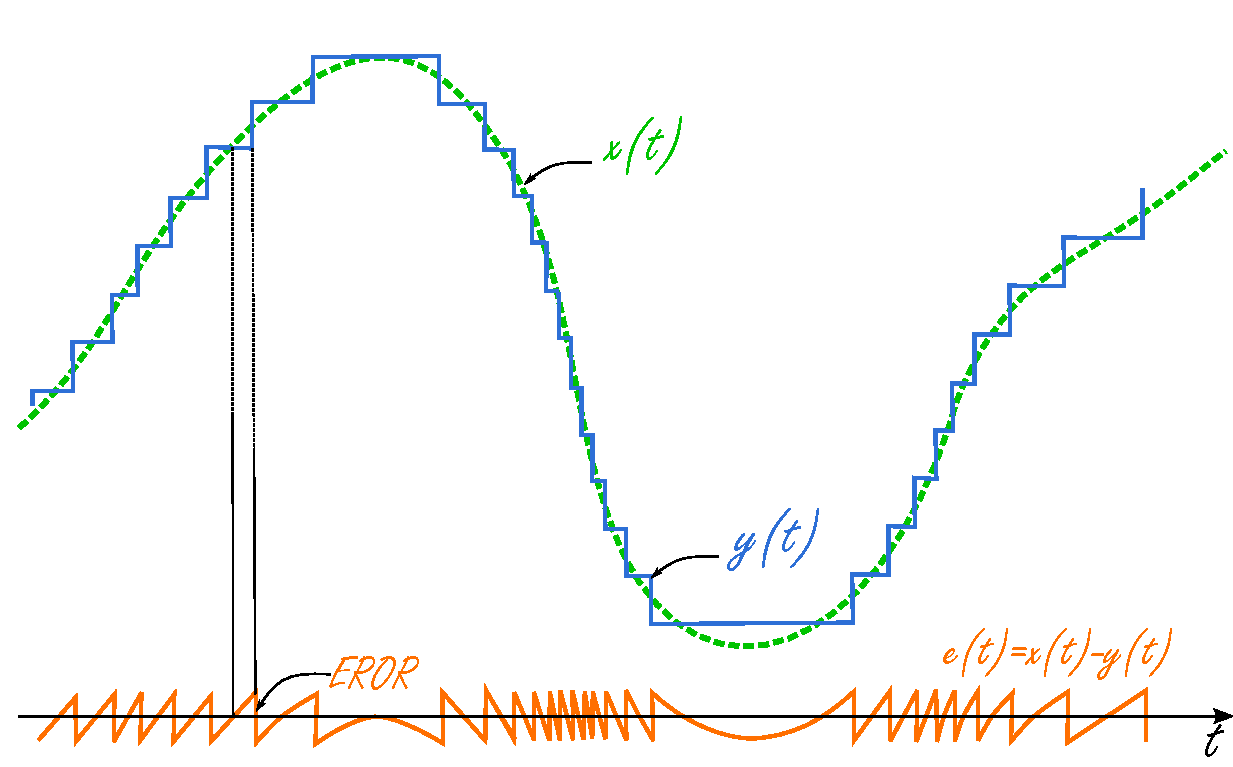
\includegraphics[width=1\linewidth]{Quantized_signal_wave.pdf}
         \caption[Kvantizační chyba]{Kvantizační chyba je rovna rozdílu původního x(t) a kvantovaného signálu v úrovni y(t) \cite{Bennett}}
         \label{AES:fig_Quntized_sig_wave}
       \end{figure}

       %The quantization error for any ac signal which spans more than a few LSBs can be approximated by an   
       %uncorrelated sawtooth waveform having a peak-to-peak amplitude of q, the weight of an LSB. Although 
       %this analysis is not precise, it is accurate enough for most applications. W. R. Bennett of Bell 
       %Laboratories analyzed the actual spectrum of quantization noise in his classic 1948

       Kvantizační chyba, jejíž průběh je na obr. \ref{AES:fig_Quntized_sig_wave}, v dynamickém režimu, tj. 
       při časových změnách vstupní analogové veličiny, způsobuje \textbf{kvantizační šum}. Ten lze pozorovat 
       např. tehdy, kdy čísla získaná z převodníku A/D jsou vedena do převodníku D/A a jím je analogový 
       signál rekonstruován. Rekonstruovaný signál se jeví jako signál původní, avšak se superponovaným 
       rušivým signálem. Vzájemným odečtení rekonstruovaného a původního signálu, dostaneme samostatný rušivý 
       signál, který lze podrobit analýze. \emph{Pokud je vzorkovací signál nekorelovaný se vzorkovaným 
       signálem, je možno kvantizační šum považovat za náhodný}. Vztah mezi původním signálem a
       signálem degradovaným kvantizačním šumem vyjadřuje parametr - \texttt{SNR}
       \begin{itemize}
         \item SNR  - Signal to Noise Ratio: poměr signálu k šumu
             \begin{equation}\label{AES:eq_SNR}
                SNR = \frac{E\{x^2(t)\}}{E\{[y(t)-x(t)]^2\}}
             \end{equation}
                \begin{itemize}
                   \item $E\{.\} \cdots$ operátor průměrování
                   \item $x(t)   \cdots$ vstupní analogový signál
                   \item $y(t)   \cdots$ rekonstruovaný kvantovaný signál
                 \end{itemize}
       \end{itemize}
       Kvantizační chybu lze aproximovat nekorelovaným pilovým průběhem s amplitudou špička-špička rovnou 
       kvantizačnímu kroku $Q$. Ačkoliv takto provedená analýza (viz kapitola \ref{AES:kap_kv_sum}) není 
       přesná, v běžných aplikacích zcela postačuje.

       Na obr. \ref{AES:fig_AD_kvantizacni_chyba} je kvantování realizováno tak, že je zajištěna minimální 
       chyba kvantování, tj. převodník provádí operaci zaokrouhlování na nejbližší hodnotu. To znamená, že 
       např. číslo jedna bude generováno vstupem v intervalu $1\pm0,5V$, je-li \texttt{FS} rovno 8V a máme-li 
       k dispozici osm kvantizačních úrovní.

       Převodník, který má v celém intervalu předváděných vstupních hodnot konstantní kvantizační krok, se 
       též označuje jako lineární kvantizér. Převodník s přirozeným binárním kódem o \emph{N} bitech je 
       schopen na analogové straně reprezentovat \emph{n-1} ne\-nu\-lo\-vých úrovní analogové veličiny, 
       přičemž platí
       \begin{equation}\label{AES:eq_AD_kod}
          n = 2^N
       \end{equation}
       A jde-li o lineární N-bitový kvantizér, můžeme vyjádřit kvantizační krok vztahem
       \begin{equation}\label{AES:eq_kvant_krok}
          Q = \frac{FS}{n} = \frac{FS}{2^N}
       \end{equation}
       Nejvyšší úroveň vstupní veličiny \emph{A} pak bude
       \begin{equation}\label{AES:eq_A_max}
          A_{max} = \frac{n-1}{n}+\frac{Q}{2}
       \end{equation}

       V sekvenci bitů binárního čísla generovaného převodníkem se zpravidla první bit, který představuje nejvyšší binární řád, označuje \texttt{MSB} (\emph{Most Significant Bit}), tedy nejvýznamnější bit. Poslední bit, tj. bit v poloze nejnižšího řádu, má označení \texttt{LSB} (\emph{Least Significant Bit}), tedy nejméně významný bit. Je zřejmé, že \texttt{LSB} jednoznačně určuje základní krok na ose číslicového signálu. Dojde-li ke změně pouze v hodnotě \texttt{LSB}, změní se analogová hodnota právě o kvantizační krok. \texttt{LSB} tedy na analogové straně určuje rozlišovací schopnost převodníku. Např. osmibitový převodník má rozlišovací schopnost \texttt{FS/256}, tj. přibližně \texttt{0,4\%}. Je-li \texttt{FS = 2V}, musí rozlišit \texttt{8 mV}\cite[s.~203]{Neumann}.

       Vzhledem k diskretizaci hodnot původního analogového signálu při převodu A/D dochází ke \emph{kvantizačním chybám}. Je-li např. vstupní veličinou okamžité napětí $u_a$ a této hodnotě odpovídá na výstupu číslo $D$, pak kvantizační chybu $\varepsilon_q$ lze vyjádřit takto:
       \begin{equation}\label{AES:eq_kvant_chyba}
          \varepsilon_q = u_a - FS\frac{D}{2^N}
       \end{equation}

      \subsection{Kvantizační šum ideálního N-bitového ADC}\label{AES:kap_kv_sum}

      %The only errors (dc or ac) associated with an ideal N-bit data converter are those related to the sampling and quantization processes. The maximum error an ideal converter makes when digitizing a signal is $\pm 1/2 LSB$. The transfer function of an ideal N-bit ADC is shown in Figure 2.37. The quantization error for any ac signal which spans more than a few LSBs can be approximated by an uncorrelated sawtooth waveform having a peak-to-peak amplitude of q, the weight of an LSB.

      %The quantization error for any ac signal which spans more than a few LSBs can be approximated by an uncorrelated sawtooth waveform having a peak-to-peak amplitude of q, the weight of an LSB. Although this analysis is not precise, it is accurate enough for most applications. W. R. Bennett of Bell Laboratories analyzed the actual spectrum of quantization noise in his classic 1948

      V předchozí kapitole byla nastíněna možnost aproximace kvantizační chyby jaké\-ho\-koliv AC signálu v 
      časové oblasti (viz \ref{AES:fig_Quntized_sig_wave}) nekorelovaným pilovým průběhem, za cenu určité 
      nepřesnosti vyvážené jednodušším matematickým aparátem.

      Vyjděme tedy z převodní charakteristiky ideálního N-bitového převodníku zatížené kvantizační chybou, 
      tak jak je znázorněna na obr. \ref{AES:fig_AD_kvantizacni_chyba}. Z té je patrné, že chyba může v 
      absolutní hodnotě dosáhnout maximálně $e(t) = \frac{Q}{2}$, resp. $\pm\frac{1}{2}LSB$ a v rámci 
      kvantizačním kroku ji lze popsat přímkou se strmostí \texttt{s}: $$e(t) = st, 
      -\frac{Q}{2s}<t<+\frac{Q}{2s}.$$ Statisticky je pravděpodobnost jejího rozložení 1/Q a je rovnoměrná od 
      $-\frac{Q}{2}$ do $+\frac{Q}{2}$.

      \begin{figure}[ht!]
        \centering
        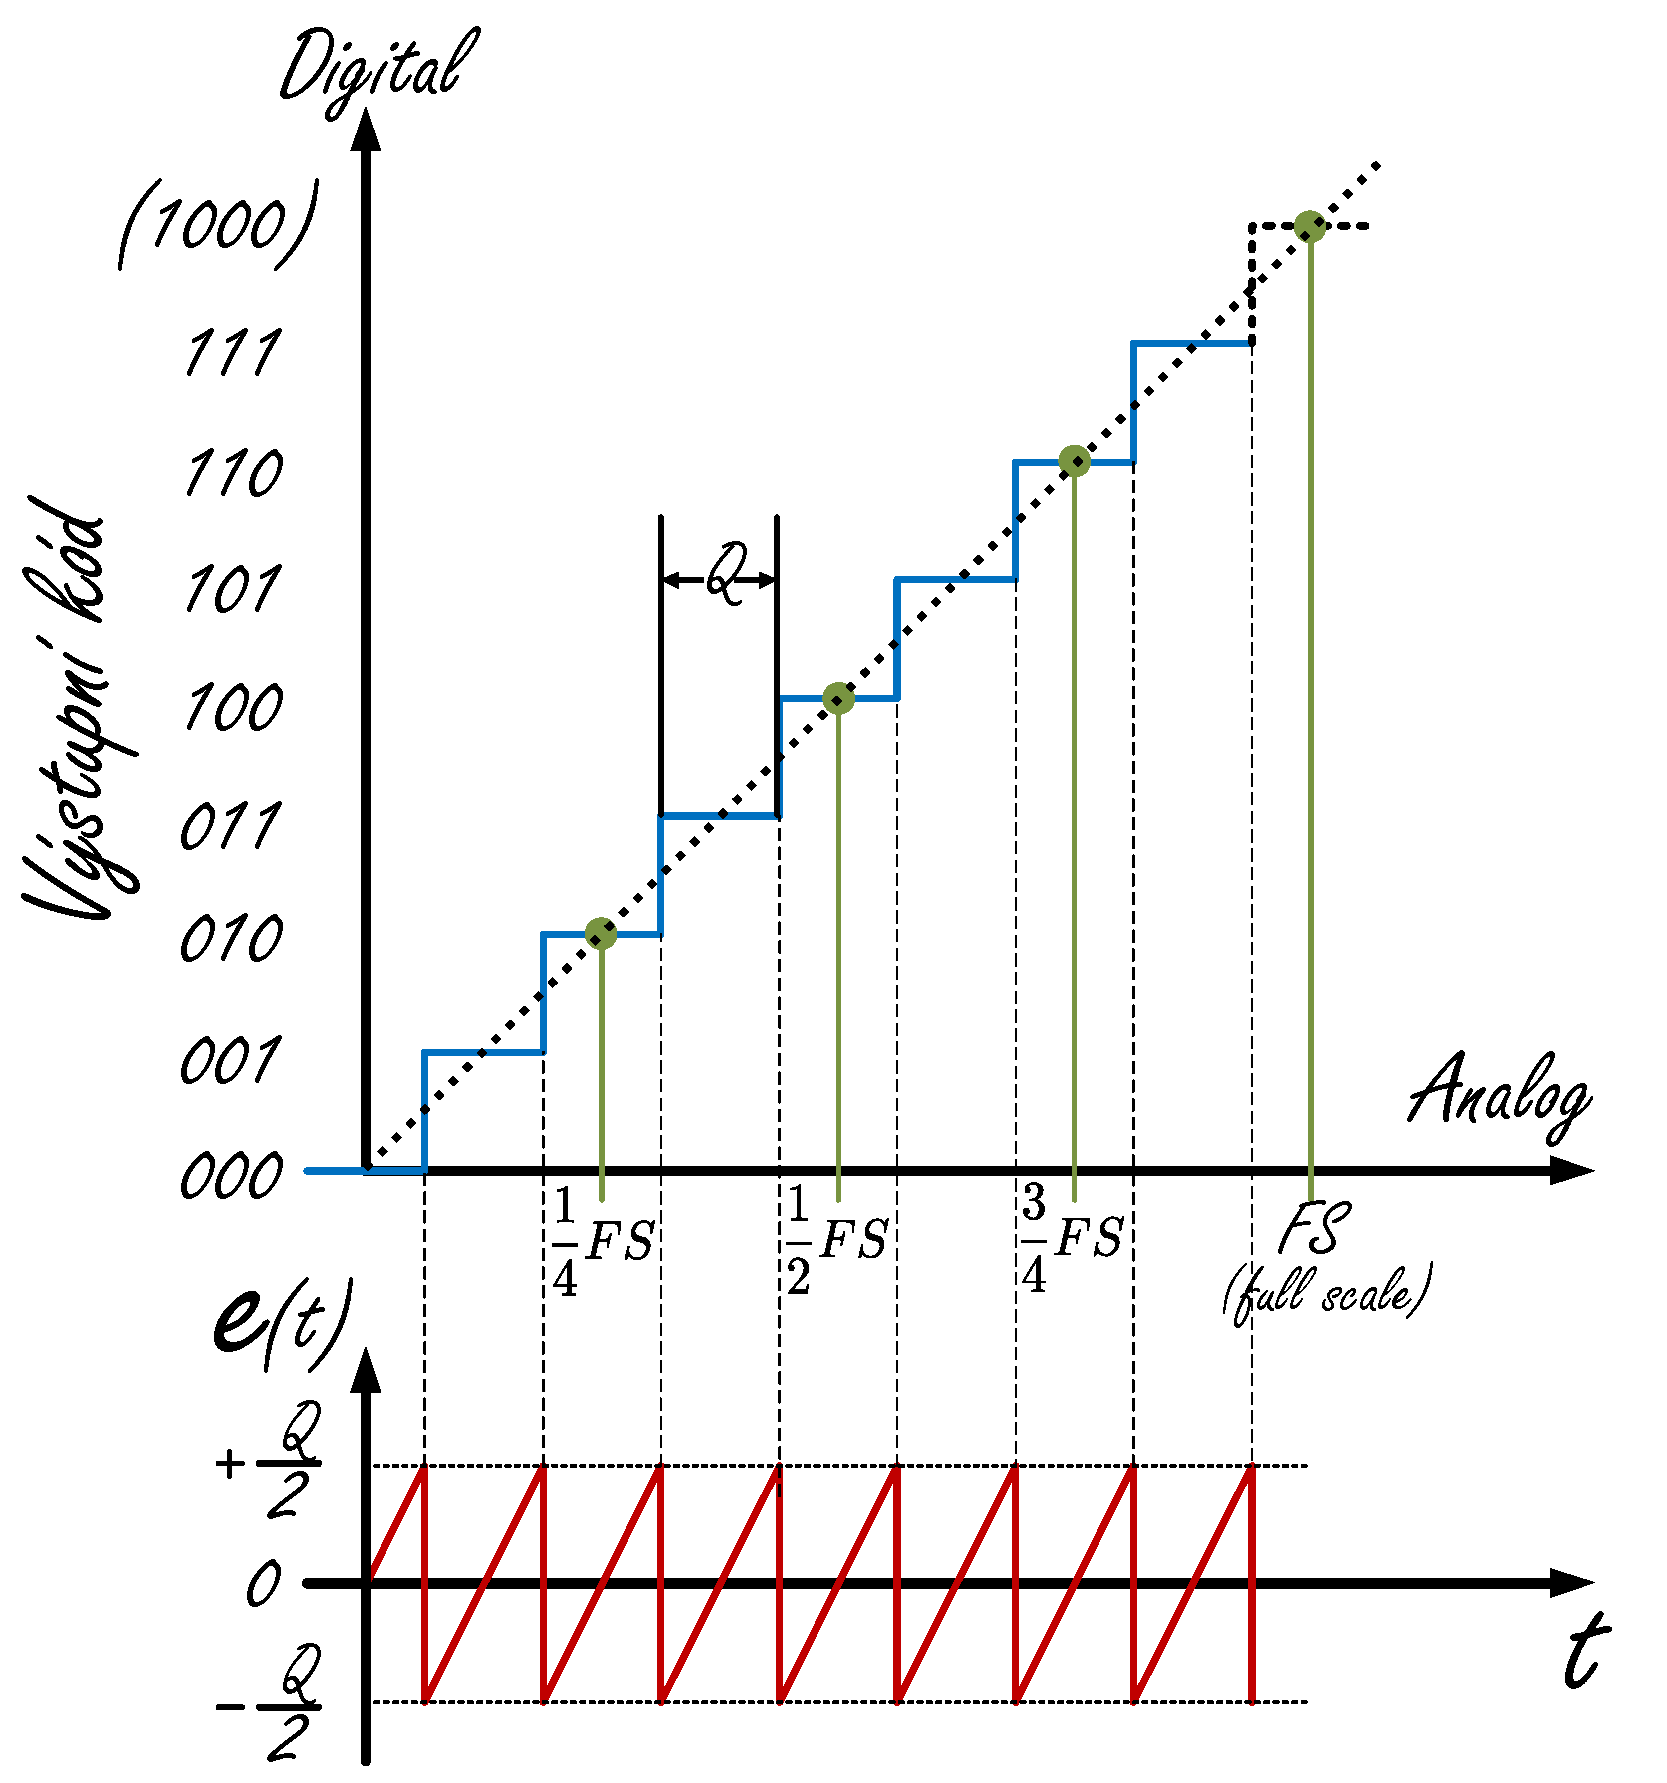
\includegraphics[width=0.8\linewidth]{AD_kvantizacni_chyba.pdf}
        \caption[Převodní charakteristika ideálních převodníků]{Převodní charakteristika ideálních převodníků a závislost chyby kvantizace na vstupní analogové hodnotě}
        \label{AES:fig_AD_kvantizacni_chyba}
      \end{figure}

      Z výše uvedeného plyne, že okamžitá hodnota kvantizační chyby $\varepsilon_q(t) = y(t) - x(t)$ může dosáhnout rozkmitu maximálně $\pm \frac{Q}{2}$ a jelikož předpokládáme rovnoměrné rozložení hodnot, je hustota pravděpodobnosti amplitud rovna $\frac{1}{Q}$.

      \emph{Kvantizační šum $\sigma^2$ je definován jako výkon (rozptyl) střídavé složky kvantizační chyby $\varepsilon_q$ a jeho efektivní hodnotu $\sigma$ můžeme odvodit pomocí věty o druhém centrálním momentu nebo výpočtem efektivní hodnoty v časové oblasti.}

        \begin{figure}[ht!]
          \centering
          \subfloat[Hustota pravděpodobnosti kvantizačního šumu]{\label{AES:fig_kvant_sum1}
            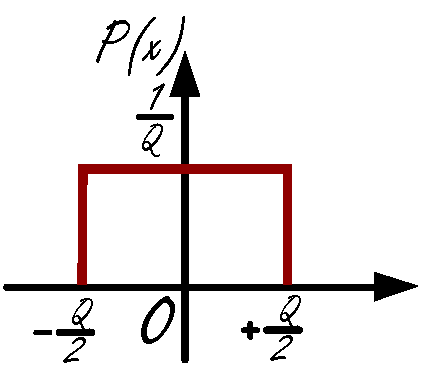
\includegraphics[width=0.4\linewidth]{AD_kvantizacni_sum1.pdf}}
          \subfloat[Kvantizační šum jako funkce času]{\label{AES:fig_kvant_sum2}
            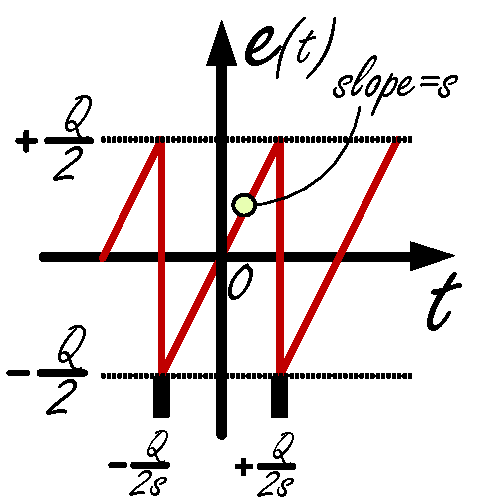
\includegraphics[width=0.4\linewidth]{AD_kvantizacni_sum2.pdf}}
          \caption{K odvození efektivní hodnoty kvantizačního šumu}
          \label{AES:fig_kvant_sum}
        \end{figure}

        \begin{enumerate}
          \item V pravděpodobnostním počtu je K-tý moment definován jako: $$M_k = \int_{-\infty}{^\infty} 
                x^k p(x)dx$$ tedy $$e(t) = \int_{-\frac{Q}{2}}^{+\frac{Q}{2}}(x - x_0)^2p(x)dx = 
                \frac{1}{Q}\int_{-\frac{Q}{2}}^{+\frac{Q}{2}}x^2dx = \frac{Q^2}{12}$$
          \item V časové oblasti má kvantizační šum pilový průběh viz obr. \ref{AES:fig_kvant_sum2}. Z  
                definičního integrálu efektivní hodnoty dostaneme $$ \overline{e^2(t)} = 
                \frac{s}{Q}\int_{-\frac{Q}{2}}^{+\frac{Q}{2}}(st)^2dt = \frac{Q^2}{12}.$$ Též můžeme využít 
                znalosti efektivní hodnoty pro průběh tohoto typu: $\frac{U_m}{\sqrt{3}}$ a dosazením za $U_m 
                =\frac{Q}{2}$ získáme opět stejný výsledek jako při výpočtu integrálu
        \end{enumerate}

        Tedy efektivní hodnota kvantizačního šumu ideálního N-bitového převodníku je:
        \begin{equation}\label{AES:eq_ef_kv_sumu}
            e(t) = \frac{Q}{\sqrt{12}}
        \end{equation}
        Předpokládejme na vstupu převodníku ustálený harmonický signál o amplitudě $X$. Dále předpokládejme, že signál s amplitudou $X_m$ by pokryl celý rozsah 
        převodníku $FS$. Pak se dá ze vztahu \ref{AES:eq_SNR} vyjádřit odstup signálu od šumu \texttt{SNR} ideálního \emph{N-bitového} převodníku jako podíl 
        jejich výkonů resp. kvadrátu efektivních hodnot signálu a šumu v decibelech vztahem
        \begin{align}
          SNR      &= \frac{P_{signal}}{P_{noise}} = \left(\frac{A_{signal}}{A_{noise}}\right)^2         \\
          SNR_{dB} &= 10\log\frac{P_{signal}}{P_{noise}} = 10\log\left(\frac{A_{signal}}{A_{noise}}\right)^2 = 20\log\frac{A_{signal}}{A_{noise}} \\
        \end{align}
        \begin{equation}\label{AES:eq_SNR_N}
            SNR  = 1,76 + 6,02N + 20log\left(\frac{X}{X_m}\right)
        \end{equation}

        Lze tedy říci, že každý bit navíc v digitálním výstupu A/D převodníku přinese zlepšení odstupu signálu od šumu o \texttt{6 dB}. Naproti tomu je třeba vědět, že uvedený výraz počítá s harmonickým signálem různého rozkmitu. Při zmenšování amplitudy bude relativní podíl šumu v signálu vyšší. Poměry se také mohou velmi změnit, když signál nebude mít harmonický charakter.

      \subsubsection{Odstup signálu od šumu}\label{AES:cap_SNR}
        Z předchozí kapitoly víme, že SNR je definován jako poměr výkonu signálu k výkonu šumu ($v\acute{y}kon = ef. hodnota^2$). Pro samotný kvantizační šum platí:
        \begin{align}
          SNR_{dB} &= 10\log\left(\frac{\dfrac{2^N}{2\cdot\sqrt{2}}\cdot Q}{\dfrac{Q}{\sqrt{12}}}\right)^2 = N20\log2 + 20\log\frac{\sqrt{12}}{2\cdot\sqrt{12}} \\ \nonumber
          SNR_{dB} &= 6,02\cdot N + 1,76dB
        \end{align}

        \begin{figure}[ht!]
            \centering
            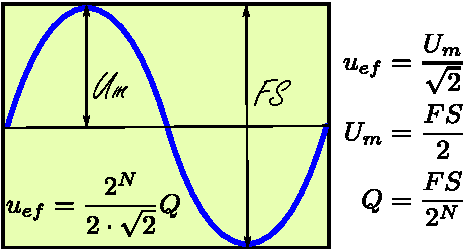
\includegraphics[width=0.6\linewidth]{AD_SNR.pdf}
            \caption{}
            \label{AES:fig_SNR}
        \end{figure}

        Tato hodnota platí pouze pro ideální převodník pouze s kvantizační chybou, a sinusový signál s rozkmitem přes celý rozsah převodníku.  Skutečný převodník má ovšem vlivem dalších chyb \texttt{SNR} menší než \texttt{SNR} určený pouze pro kvantizační šum. Tato hodnota se nazývá \texttt{SINAD} nebo \texttt{SNDR} - \emph{Signal-to-Noise and Distortion ratio}.

        Známe-li \texttt{SNR} skutečného převodníku, můžeme určit počet efektivních bitu $N_{ef}$ tzn. \emph{efektivní rozlišitelnost převodníku}. Ten je vždy menší než $N$.
        \begin{equation}\label{AES_eq_N_ef}
            N_ef = \frac{SNR - 1,76}{6,02}
        \end{equation}
        
  \section{Principy A/D převodníků}
      Převod analogového signálu na číslo lze uskutečnit několika různými postupy:\cite{Neumann}
      \begin{enumerate}
        \item Vstupní signál se porovnává s kvantovanou referenční veličinou a komparátory okamžitě 
              vyhodnotí, který z nich je větší. Přímým výstupním údajem je binární číslicové slovo.
        \item Vstupní signál i referenční veličina se v určité časové sekvenci zavádějí do integrátoru a  
              komparátor na jeho výstupu určuje sekvenci
              impulsů, vypovídající o hodnotě vstupní analogové veličiny. Informací o vstupní veličině dále 
              přenáší počet impulsu, jejich kmitočet nebo kódovaná sekvence impulsů. Tato informace může být 
              převedena číslicovým blokem (obvykle blokem DSP) na binární číslicové slovo.
      \end{enumerate}

      Bývá také používáno třídění na \emph{převodníky s přímým a nepřímým vyhodnocení analogové veličiny}.
      \begin{itemize}
        \item \texttt{Převodníky s přímým vyhodnocením} porovnávají hodnoty analogové veličiny s vybranými  
              kvantizačními úrovněmi současně nebo postupně, a to tak, že každá úroveň má vlastní komparátor. 
              K těmto převodníkům patří \emph{převodníky paralelní a kaskádní}.
        \item \texttt{K nepřímému převodu} můžeme využít postupného provoláváním vstupní ve\-li\-či\-ny s  
              vhodnými vzorky referenčního napětí, dodávanými na vstup jediného komparátoru v pořadí a 
              velikosti řízené logickými obvody. U těchto převodníků je vstupní analogová veličina
              porovnávaná s výstupní veličinou převodníku \texttt{D/A}, přičemž je číslicový vstup tohoto 
              převodníku měněn tak, aby se obě veličiny k sobě přibližovaly. Pokud se k sobě dostatečně 
              přiblíží, je převod ukončen. I zde jsou v podstatě jen dvě jednoduché možnosti
              přibližování výstup převodníku \texttt{D/A} k určité úrovni vstupní veličiny: buď se 
              přibližování děje se stálým krokem, kdy jde o krokování po jednotlivých kvantovacích úrovních 
              (\emph{převodníky sledovací}), nebo postupnou aproximací (\emph{převodníky aproximační}), kdy 
              první krok rozhoduje o hodnotě \texttt{MSB}, další kroky porovnávají binárně zmenšované hodnoty 
              odpovídající jednotlivým binárním řádům s tím, že poslední krok určí hodnotu \texttt{LSB}.
        \item Jinou možností nepřímého převodu A/D je převést hodnotu vstupní veličiny na takový parametr  
              pomocného signálu, který se pak dá snadno převést na číslicový údaj. Tímto parametrem je 
              nejčastěji kmitočet, jindy to může být i počet impulzů v určitém časovém intervalu nebo
              kódovaná sekvence impulzů. U těchto převodníků j kromě komparátoru typickým funkčním blokem integrátor.
      \end{itemize}

  \section{Převod číslicového signálu na analogový}
    Číslicově-analogové převodníky převádějí číslicový signál zpravidla ve formě binárně kódovaného čísla na proud nebo napětí.
    \begin{equation}\label{AES_eq_DA}
        U_A = D \cdot U_{REF} \quad  I_A = D \cdot I_{REF}
    \end{equation}
    kde $U_{REF}, I_{REF}$ jsou referenční napětí a proud určující rozsah výstupní veličiny. Je-li referenční 
    napětí konstantní jedná se o klasické převodníky \texttt{DAC}. Při proměnném referenčním napětí se jedná 
    o násobící převodníky \texttt{MDAC}, které realizují násobení časově proměnného referenčního spojitého a 
    vstupního číslicového signálu.  Hodnota číslicového signálu $D$ se vyjadřuje ve dvojkovém nebo dvojkově
    desítkovém (\texttt{BCD}) kódu.
    Ve dvojkovém kódu:
    \begin{equation}\label{AES:eq_DA_Dbin}
        D_B =\sum_{i=1}^n a_i\cdot2^{-i}
    \end{equation}
    $n$ je počet bitů dvojkového čísla. Bit $a_1$ s nejvyšší vahou $1/2$ se označuje \textbf{MSB}, bit  $a_n$ 
    s nejnižší vahou $2^{-n}$  se označuje \textbf{LSB}. \emph{Maximální hodnota číslicového signálu $D_{MAX} 
    = 1 - 2^{-n}$ a proto maximální hodnota výstupní veličiny je vždy o 1 LSB menší, než je rozsah 
    převodníku.} Veličina $2^{-n}\cdot U_{REF}$, resp. $2^{-n}\cdot I_{REF}$ se nazývá \textbf{kvantum 
    referenčního napětí nebo proudu} a určuje \textbf{rozlišitelnost} převodníku. Převodní funkci D/A 
    převodníku můžeme v případě binárního kódu vyjádřit vztahem
    \begin{equation}\label{AES:eq_DA_bin}
        U_A = U_{REF}\cdot\left(a_{n}2^{-n} + a_{n-1}2^{-(n-1)} + \cdots + a_12^{-1}\right)
    \end{equation}
    Statické vlastnosti \texttt{D/A} převodníku jsou určeny převodní charakteristikou, která je obvykle 
    lineární (obr. \ref{AES:fig_DA_prevodni_charka}). Převodní charakteristika reálného DA převodníku je 
    zatížena chybou nuly, chybou zisku, integrální a diferenciální nelinearitou a monotónností převodu.

    Z převodní charakteristiky lze tedy určit následující parametry převodníku:
    \begin{itemize}
      \item Chybu nuly (posunu) $\varepsilon_0$
           \begin{equation}\label{AES_eq_chyba_nuly}
             \varepsilon_0 = \frac{\Delta U_0}{U_{REF}}
           \end{equation}
      \item Chybu měřítka (zesílení) $\varepsilon_m$
           \begin{equation}\label{AES_eq_chyba_zesileni}
             \varepsilon_m = \frac{\Delta U_m - \Delta U_0}{U_{REF}}
           \end{equation}
      \item Integrální nelinearitu $I_{NL}$ jako maximální odchylku výstupního napětí sku\-teč\-né\-ho 
      převodníku od ideální hodnoty v celém rozsahu převodníku
           \begin{equation}\label{AES_eq_chyba_integralni}
             I_{NL} = \frac{\max\Delta U_n}{U_{REF}}
           \end{equation}
    \end{itemize}

    \begin{figure}[ht!]
       \centering
       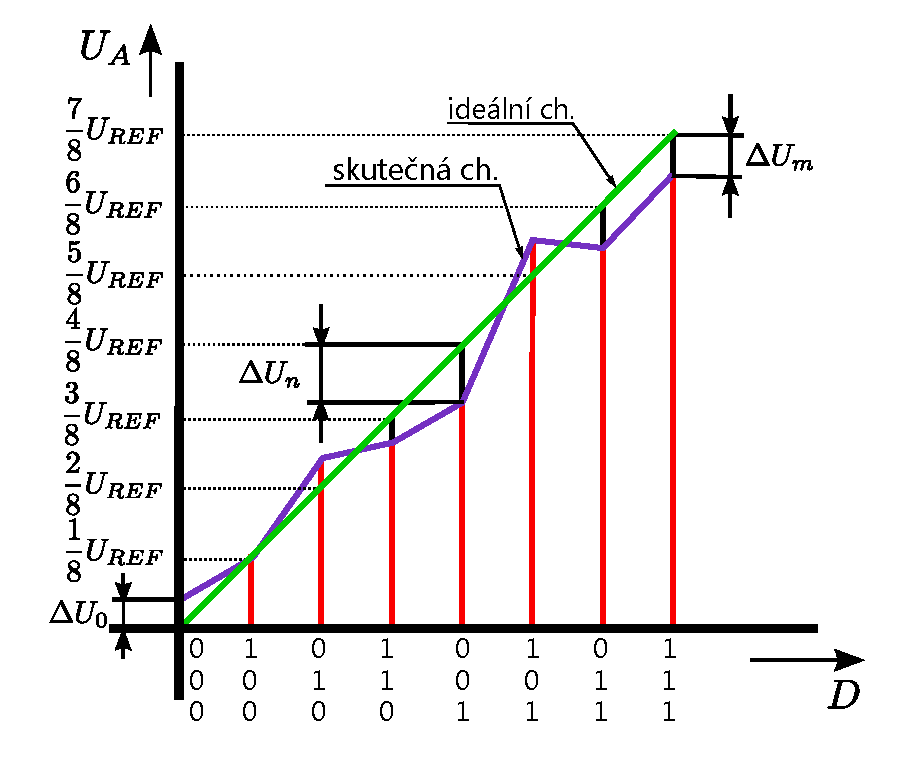
\includegraphics[width=1\linewidth]{DA_prevodni_charka.pdf}
       \caption[Převodní charakteristika DA převodníku]{Statická převodní charakteristika 3 bitového DA převodníku}
       \label{AES:fig_DA_prevodni_charka}
    \end{figure}

    Všechny tyto chyby se vyjadřují buď v procentech jmenovitého rozsahu $U_{REF}$ pře\-vod\-ní\-ku, nebo v 
    jednotkách ideální kvantizační úrovně (kvanta) $q = 2^{-n}\cdot U_{REF}$.

    Dynamické vlastnosti D/A převodníku jsou charakterizovány \textbf{dobou ustálení} $T_u$ (obr. 
    \ref{AES:fig_DA_Tu}), potřebnou k ustálení výstupního signálu na jmenovitou hodnotu se zadanou chybou 
    $\Delta U$ obvykle $\pm0.5 LSB$.

    U násobících D/A převodníků se navíc určuje kmitočtový rozsah referenčního napětí kmitočtem $f_m$, při 
    kterém poklesne výstupní napětí převodníku o $3 dB$ oproti stejnosměrnému napětí při maximální hodnotě 
    číslicového signálu.

    \begin{figure}[ht!]
       \centering
       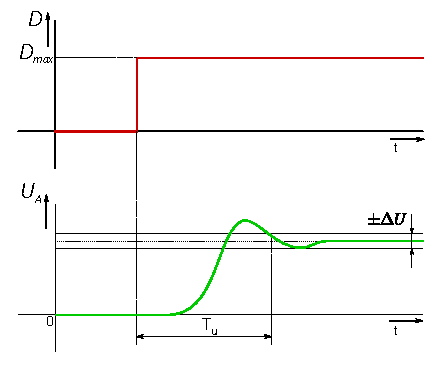
\includegraphics[width=0.4\textwidth]{DA_doba_Tu.pdf}
       \caption[Doba ustálení DA převodníku]{Doba ustálení $T_a$ DA převodníku. Je to celková doba od změny vstupního kódu do ustálení analogového výstupu s přesností $\pm\frac{1}{2}LSB$}
       \label{AES:fig_DA_Tu}
    \end{figure}

    \subsection{DA převodník DAC0800}
      D/A převodník DAC0800 je velmi rychlý násobící D/A převodník s rozlišením 8 bitů, pracující na principu 
      spínaných proudových zdrojů (viz obr. \ref{AES:fig_DAC0800_blok_sch}).
      \begin{figure}[ht!]
        \centering
        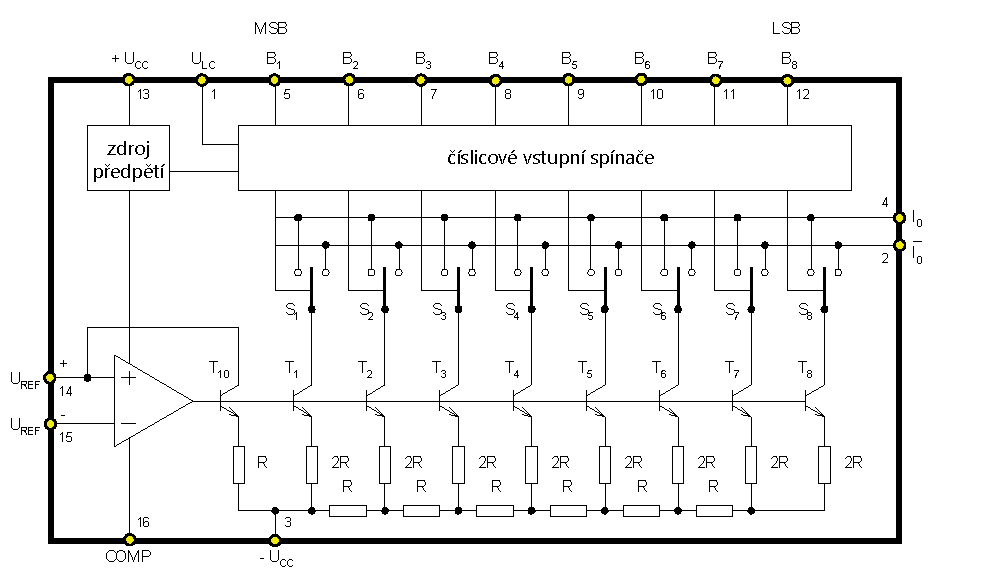
\includegraphics[width=1\linewidth]{DAC0800_block_diagram.pdf}
        \caption[Blokové schéma DAC0800]{Blokové schéma DA převodníku DAC0800}
        \label{AES:fig_DAC0800_blok_sch}
      \end{figure}

      Vstup převodníku je proudový, proudový výstup je řešen jako komplementární. IO v sobě slučuje proudové 
      spínače, váhové odpory a řídící zesilovač. Analogová reference, přesné vnější odpory, korekční 
      kondenzátor a výstupní zesilovač se připojují vně převodníku. Převodník \texttt{DAC0800} generuje 
      váhové proudy do komplementárních proudových sběrnic $I_0$ a $\overline{I}_0$ prostřednictvím spínaných 
      proudových zdrojů s tranzistory $T_1$ až $T_8$ a odporovou sítí $R-2R$ viz obr. 
      \ref{AES:fig_DAC0800_blok_sch}. Při úrovni \texttt{H} na číslicových vstupech $B_1$ až $B_8$ připojí 
      spínače $S_1$ až $S_8$ příslušné váhové proudy na výstup $I_0$ a při úrovni \texttt{L} na výstup 
      $\overline{I}_0$.

      Nezávislost váhových proudů na teplotních změnách zajišťuje referenční zdroj prou\-du s tranzistorem 
      $T_{10}$ a zesilovačem \texttt{Z}, ke kterému se připojuje referenční proud o jmenovité hodnotě $2 mA$. 
      Kondenzátor s kapacitou $10 nF$ připojený mezi vývody \texttt{3} a \texttt{16} slouží ke kmitočtové 
      kompenzaci zesilovače \texttt{Z}. Číslicové vstupy $S_1$ až $B_8$ řídí spínače $S_1$ až $S_8$ 
      prostřednictvím převodníku úrovní, přičemž svorkou $V_{LC}$ (pin 1) lze volit slučitelnost převodníku s 
      obvody TTL, DTL, CMOS atd.

      Vstupní referenční proud $I_{REF}$ je odvozen pomocí vnějšího přesného odporu $R_{REF}$ ze zdroje 
      referenčního napětí $U_{REF}$. Souběh referenčního proudu a plného výstupního proudu $I_{FS}$ je 
      zachován v rozpětí dvou dekád proměnné unipolární reference a umožňuje použít IO též jako násobící 
      převodník. Výstupní proudy $I_0$, $\overline{I}_0$ z vysokoimpedančních výstupů se mohou využívat přímo 
      nebo pomocí vnějších odporů, popřípadě pomocí \texttt{OZ}, se mohou převést na napětí. Převodník 
      pracuje se vstupním přímým binárním kódem při využití přímého proudového výstupu $I_0$ nebo se vstupním 
      komplementárním binárním kódem, využije-li se doplňkový proudový výstup $\overline{I}_0$. Rozhodovací
      úroveň číslicových vstupů lze z vnějšku nastavit na potřebnou hodnotu. Proto lze k řízení převodníku 
      \texttt{DAC0800} použít všechny běžně používané řady log. obvodů.

      \begin{figure}[ht!]
        \centering
        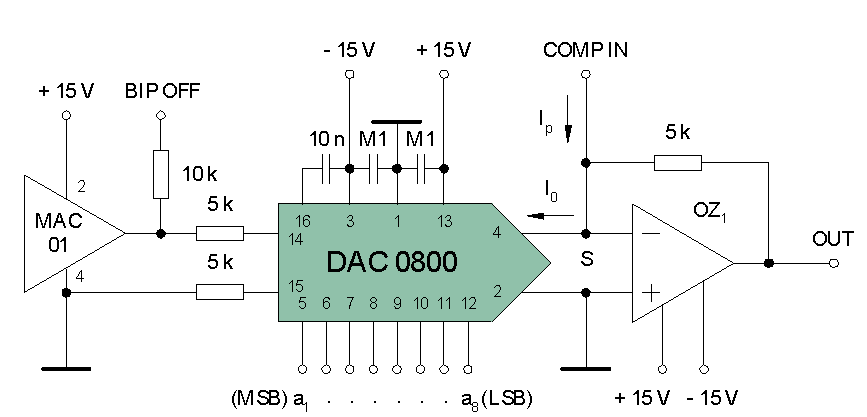
\includegraphics[width=1\linewidth]{DAC0800_sch1.pdf}
        \caption[Zapojení převodníku DAC0800]{Příklad zapojení převodníku DAC0800}
        \label{AES:fig_DAC0800_sch1}
      \end{figure}

      Příklad zapojení D/A převodníku je na obr. \ref{AES:fig_DAC0800_sch1}. Obsahuje kromě vlastního D/A 
      převodníku \texttt{DAC0800} zdroj referenčního napětí \texttt{MAC01} se jmenovitým referenčním napětím 
      +10 V a invertor se zesilovačem, pracujícím ve funkci převodníku proudu na napětí pro realizaci 
      napěťového výstupu převodníku. Funkce je následující: Napětí $+10 V$ z \texttt{ MAC01} je pomocí odporu 
      $5k\Omega$ převedeno na proud $I_{REF} = 2 mA$, který je přiveden do kladného referenčního vstupu 
      \texttt{DAC0800}, kde je vynásoben nastavenou hodnotou číslicového signálu, zadanou pomocí osmi 
      dvoupolohových přepínačů. Poté se proud max $-2\cdot\left(1 - 2^{-8}\right) mA$ objeví na výstupu $I_0$ 
      a invertující zesilovač převede na odpovídající napětí. Zpětnovazební rezistor zesilovače $5k\Omega$ 
      určuje rozsah výstupního napětí 0 až 10 V (unipolární režim). Jsou-li svorky \texttt{BIP OFF} a 
      \texttt{COMP IN} propojeny, pak do sčítacího bodu \emph{S} je přiveden proud $I_p = I_{REF}/2$ tj. 1 mA 
      ($I_p = 10 V/10 k\Omega$) opačného směru než $I_0$, který způsobí trvalý posun výstupní napěťové úrovně 
      převodníku o $-5 V$, takže rozsah převodníku bude $\pm5 V$ (bipolární režim) a hodnota výstupního 
      napětí je určena dvojkovým kódem s posunutím (MSB určuje polaritu výstupního napětí).
